\documentclass{article}

\usepackage{amsfonts}
\usepackage{amsmath}
\usepackage{interval}
\usepackage[T1]{fontenc}
\usepackage{pdftexcmds}
% \usepackage{minted}
\usepackage{pgfplots}
\pgfplotsset{compat=1.8}

\renewcommand*{\mathellipsis}{%
  \mathinner{{\ldotp}{\ldotp}{\ldotp}}%
}

\begin{document}

\title{A Model of Double-Entry Bookkeeping Systems}
\author{}
\date{}
\maketitle

\section{Double-Entry Bookkeeping Space}

We can view a double-entry bookkeeping information system as a 
three dimensional space $S=\{(a,d,m)\mid a\in A, d\in D, m\in M\}$, where,

\begin{itemize}
	\item $A$ is a finite ordered subset of a predefined set of accounts.
	\item $D$ is a finite ordered subset of all 
		possible dates in the Gregorian calendar.
	\item $M$ is a finite ordered subset of all 
		possible discrete moments in time, given a precision.
\end{itemize}

Figure~\ref{fig:deb-space-sample} shows a \emph{double-entry bookkeeping space} sample, 
where each cube represents a tuple of the form $(a,d,m)$ and is associated with
a integer value different from zero.
Consider the cubes $(4,1,1)$ and $(6,1,1)$. They share the same moment 
and date---the only difference are the accounts. 
We can interpret this pair of cubes as a transaction recorded in the system,
with one cube representing the debit and another representing the credit.

\begin{figure}[h]
\centering
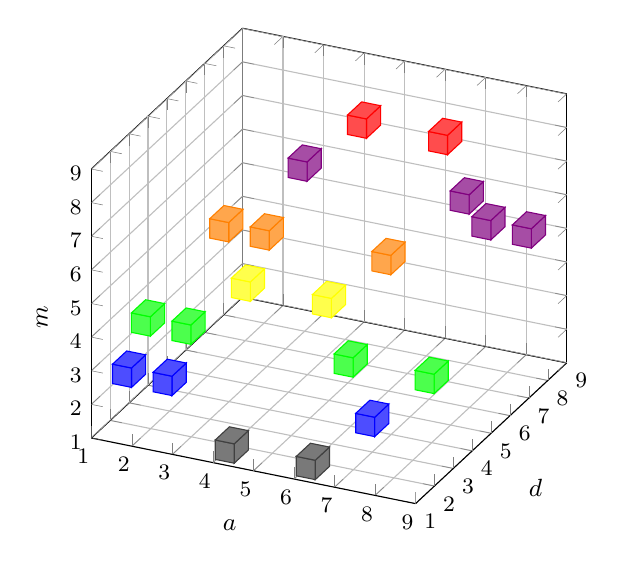
\begin{tikzpicture}
\begin{axis}[
	% view={120}{40},
	small,
	height=3in,
	width=3in,
	grid=major,
	xlabel=$a$,
	ylabel=$d$,
	zlabel=$m$,
	xmin=1,xmax=9,
    ymin=1,ymax=9,
    zmin=1,zmax=9,
    xtick={1,2,...,10},
    ytick={1,2,...,10},
    ztick={1,2,...,10},
	colormap={summap}{
        color=(darkgray); color=(blue);
        color=(green); color=(yellow)
        color=(orange) color=(violet)
        color=(red)
    },
    scatter/use mapped color={
        draw=mapped color,fill=mapped color!70},
]
\addplot3[only marks,scatter,mark=cube*,mark size=7] coordinates {
            (4,2,1) (6,2,1) 
            (7,3,2) (1,3,2) (2,3,2)
            (1,4,3) (2,4,3) (6,4,3) (8,4,3)
            (3,5,4) (5,5,4) 
            (3,6,5) (6,6,5) (2,6,5)
            (8,7,6) (9,7,6) (3,8,6) (7,8,6)
            (4,9,7) (6,9,7)
        };
\end{axis}
\end{tikzpicture}
\label{fig:deb-space-sample}
\caption{A \emph{double-entry bookkeeping space} sample.}
\end{figure}

As, by definition, a double-entry transaction must have debits' sum
equals to credits' sum, we can deduce that the values for both
cubes $(4,1,1)$ and $(6,1,1)$ are the same, in this example.

More specifically, we can represent a \emph{double-entry bookkeeping space} 
as a three dimensional array $S$:
\begin{equation}
	\label{eq:space}
	S = \left(s_{ijk}\right), where
	\; 1 \leq i \leq |A|, \; 1 \leq j \leq |D|, \; 1 \leq k \leq |M|, 
	\; s_{ijk} \in \mathbb{Z}
\end{equation}

Satisfying the following property:

\begin{equation}
	\label{eq:property}
	\forall j, k\left(\sum_{i=1}^{|A|}{s_{ijk}} = 0\right)
\end{equation}

In equations~\eqref{eq:space}~and~\eqref{eq:property}
we assume that debits are represented by positive integers
and credits by negative integers.

\section{Operations}

In the following description of the operations, the notation $\langle x, y \rangle$ means
a range specification, and $R^{\langle n \rangle}$ means a set of $n$
range specifications based on the ordered set $R$.

A \emph{double-entry bookkeeping space} supports the following operations:

\begin{description}
	\item[\textsc{Append}$(S,S')$] append the space
	$S'=\left(s'_{ijk}\right)$ to the space $S$,
		such that, exists a set $M$ which is associated with both space $S$ and
		space $S'$. Let $k_1$ be the maximum value of $k$, such that
		$s_{ijk} \neq 0$, and let $k_2$ be the minimum value of $k$,
		such that $s'_{ijk} \neq 0$. Given that $k_1 < k_2$, then:
		\[
			\forall i,j\left(s_{ijk} = s'_{ijk}\right), where \; k_2 \leq k \leq |M|.
		\]

	\item[\textsc{Projection}$(S, A', D^{\langle n \rangle}, M^{\langle m \rangle})$] 
		returns another space $S'=\left(s'_{ijk}\right)$,
		where $A' \subseteq A$, and $D^{\langle n \rangle} = 
		\{\langle x_1, y_1 \rangle, \ldots, \langle x_n, y_n \rangle\}$, and
		$M^{\langle m \rangle} = 
		\{\langle v_1, w_1 \rangle, \ldots, \langle v_m, w_m \rangle \}$, and
		for all distinct $\langle x_i, y_i \rangle$ and $\langle x_j, y_j \rangle$,
		$\{x_i,\ldots,y_i\} \cap \{x_j,\ldots,y_j\} = \emptyset$, and
		for all distinct $\langle v_i, w_i \rangle$ and $\langle v_j, w_j \rangle$,
		$\{v_i,\ldots,w_i\} \cap \{v_j,\ldots,w_j\} = \emptyset$. Then:
		\[
			s'_{ijk} = 
			\begin{cases}
				\sigma_{ijk}, & 
					\text{if } f(j, k) \neq \emptyset \land 
						D_j \in X \land M_k \in V \\
				0, & \text{otherwise},
			\end{cases} \\
		\]
		where:
		\begin{align*}
			\sigma_{ijk} &= \sum_{p=j}^{j+|x_r, \ldots, y_r|-1} \;
				{\sum_{q=k}^{k+|v_s, \ldots, w_s|-1}{s_{ipq}}}, \\
			X &= \{ x_1, \ldots, x_n \}, \\
			V &= \{ v_1, \ldots, v_m \}, \\
			x_r &= D_j, \\
			v_s &= M_k, \\
			f(j,k) &= \{ A_i : \sigma_{ijk} \neq 0 \} \cap A', \; 1 \leq i \leq |A|.
		\end{align*}

	\item[\textsc{Slice}$(S, A', D^{\langle n \rangle}, M^{\langle m \rangle})$] 
		returns another space $S'=\left(s'_{ijk}\right)$, 
		where $A' \subseteq A $, and $D^{\langle n \rangle} = 
		\{\langle x_1, y_1 \rangle, \ldots, \langle x_n, y_n \rangle\}$, and
		$M^{\langle m \rangle} = 
		\{\langle v_1, w_1 \rangle, \ldots, \langle v_m, w_m \rangle \}$,
		such that:
		\[
			s'_{ijk} = 
			\begin{cases}
				s_{ijk}, & \text{if } 
					f(j, k) \neq \emptyset \land
					D_j \in \bigcup\limits_{p=1}^{n} \{ x_p, \ldots, y_p \} \land 
					M_k \in \bigcup\limits_{q=1}^{m} \{ v_q, \ldots, w_q \} \\
				0, & \text{otherwise},
			\end{cases}
		\]
		where:
		\[
			f(j,k) = \{ A_i : s_{ijk} \neq 0 \} \cap A', \; 1 \leq i \leq |A|.
		\]

\end{description}

\section{Alloy Model} % (fold)
\label{sec:alloy_model}

% \inputminted{alloy}{model.als}%

% section alloy_model (end)

\end{document}